\documentclass[%
reprint,
amsmath,
amssymb,
aps,
bahasa,
]{revtex4-1}

\usepackage{graphicx}
\usepackage[mathletters]{ucs} % Extended unicode (utf-8) support
\usepackage[utf8x]{inputenc}
\usepackage{hyperref}
\usepackage{mhchem}

\usepackage{babel}

\begin{document}


\title{Perhitungan struktur elektronik berdasarkan teori fungsional
    kerapatan dengan fungsi basis Lagrange: Implementasi awal}
\author{Fadjar Fathurrahman}
\affiliation{Pusat Penelitian Nanosains dan Nanoteknologi, Institut Teknologi Bandung}

\begin{abstract}
This is the abstract.
\end{abstract}

\maketitle

\section{Introduction}

Welcome to \ffrLFDFT documentation.
In this document you will find the following information:
\begin{itemize}
\item basic information about \ffrLFDFT
\item how to compile and use the program
\item implementation details of the program
\end{itemize}

{\tt ffr-LFDFT} is a poor man's program (or collection of subroutines, as of now)
to carry out electronic structure calculations based on density functional theory
and Lagrange basis set.

This program is intended for research in implementation of new methods in
electronic structure calculations in condensed matter.
Currently it is not as stable of functional
as more well-known package such as Quantum Espresso, ABINIT, or VASP.
However, it can be used to calculate total energy of solids.

This program is written mainly by me, Fadjar Fathurrahman at Research Center
of Nanoscience and Nanotechnology, Bandung Institute of Technology, Indonesia.


% Add tutorial on how to use m\_LF3d module to solve Schrodinger equation
% in 1d.
% In LF3d periodic, only gamma-point sampling is used.

\section{Teori}

\cite{Choi2015,Choi2016}, 

Berdasarkan teori fungsional kerapatan,
energi total dari sistem yang terdiri dari elektron yang berinteraksi
dengan suatu potential eksternal $V_{\mathrm{ext}}(\mathbf{r})$
dapat dinyatakan sebagai
\begin{widetext}
\begin{equation}
E[\rho(\mathbf{r})] = 
-\frac{1}{2}\sum_{i}f_{i}
\int\mathrm{d}\mathbf{r}\,
\, \psi^{*}_{i}(\mathbf{r}) \nabla^2 \psi_{i}(\mathbf{r})
+ \int\mathrm{d}\mathbf{r}\,
\rho(\mathbf{r}) V_{\mathrm{ext}}(\mathbf{r})
+
\frac{1}{2}\int\mathrm{d}\mathbf{r}\,\mathrm{d}\mathbf{r}'\,
\frac{\rho(\mathbf{r})\rho(\mathbf{r}')}{\left|\mathbf{r}-\mathbf{r}'\right|}
+ E_{\mathrm{xc}}[\rho(\mathbf{r})]
\end{equation}
\end{widetext}

LDA XC:
\begin{equation}
E_{\mathrm{xc}}[\rho(\mathbf{r})] =
\int\mathrm{d}\mathbf{r}\,
\varepsilon_{\mathrm{xc}}(\rho(\mathbf{r}))
\rho(\mathbf{r})
\end{equation}

\begin{equation}
V_{\mathrm{xc}}(\mathbf{r}) = \varepsilon_{\mathrm{xc}}(\rho(\mathbf{r}))
+ \rho(\mathbf{r})\frac{\mathrm{d}\varepsilon_{\mathrm{xc}}(\rho)}{\mathrm{d}\rho}
\end{equation}

Persamaan sentral pada teori fungsional kerapatan adalah persamaan
Kohn-Sham yang dapat ditulis sebagai berikut.
\begin{equation}
\left[
-\frac{1}{2}\nabla^2
+ V_{\mathrm{Ha}}(\mathbf{r})
+ V_{\mathrm{xc}}(\mathbf{r})
+ V_{\mathrm{ext}}(\mathbf{r})
\right]\psi_{i}(\mathrm{r}) =
\epsilon_{i} \psi_{i}(\mathrm{r})
\label{eq:KS_eq}
\end{equation}
Suku potensial pertama pada persamaan $\eqref{eq:KS_eq}$,
$V_{\mathrm{Ha}}(\mathbf{r})$ menyatakan potensial Hartree,
\begin{equation}
V_{\mathrm{Ha}}(\mathbf{r}) =
\int
\frac{\rho(\mathbf{r}')}{\left|\mathbf{r} - \mathbf{r}'\right|}
\mathrm{d}\mathbf{r}'
\end{equation}
dengan $\rho(\mathbf{r})$ adalah kerapatan (muatan) elektron
yang dapat ditulis sebagai
\begin{equation}
\rho(\mathbf{r}) = \sum_{i} f_{i}\, \psi^{*}_{i}(\mathbf{r}) \psi_{i}(\mathbf{r})
\end{equation}
Suku potensial ketida adalah $V_{\mathrm{ext}}(\mathbf{r})$
yang menyatakan potensial eksternal yang dirasakan oleh elektron.

\section{Fungsi basis Lagrange}

Untuk suatu interval $[0,L_{\alpha}]$ yang diberikan, dengan $L_{\alpha} > 0$, titik grid
$x_{\alpha}$ sesuai untuk fungsi basis
Lagrange periodik dapat dinyatakan dengan persamaan berikut.
\begin{equation}
x_{\alpha} = \frac{L_{\alpha}}{2}\frac{2\alpha-1}{N_{a}}
\end{equation}
Fungsi basis Lagrange periodik yang akan digunakan
memiliki bentuk sebagai berikut.
\begin{equation}
\phi_{\alpha}(x) = \frac{1}{\sqrt{N_{\alpha}L_{\alpha}}}
\sum_{n_{\alpha}=1}^{N_{\alpha}} \cos\left[
\frac{\pi}{L_{\alpha}}(2n_{\alpha} - N_{\alpha} - 1)(x-x_{\alpha})
\right]
\end{equation}

Test
\begin{figure}
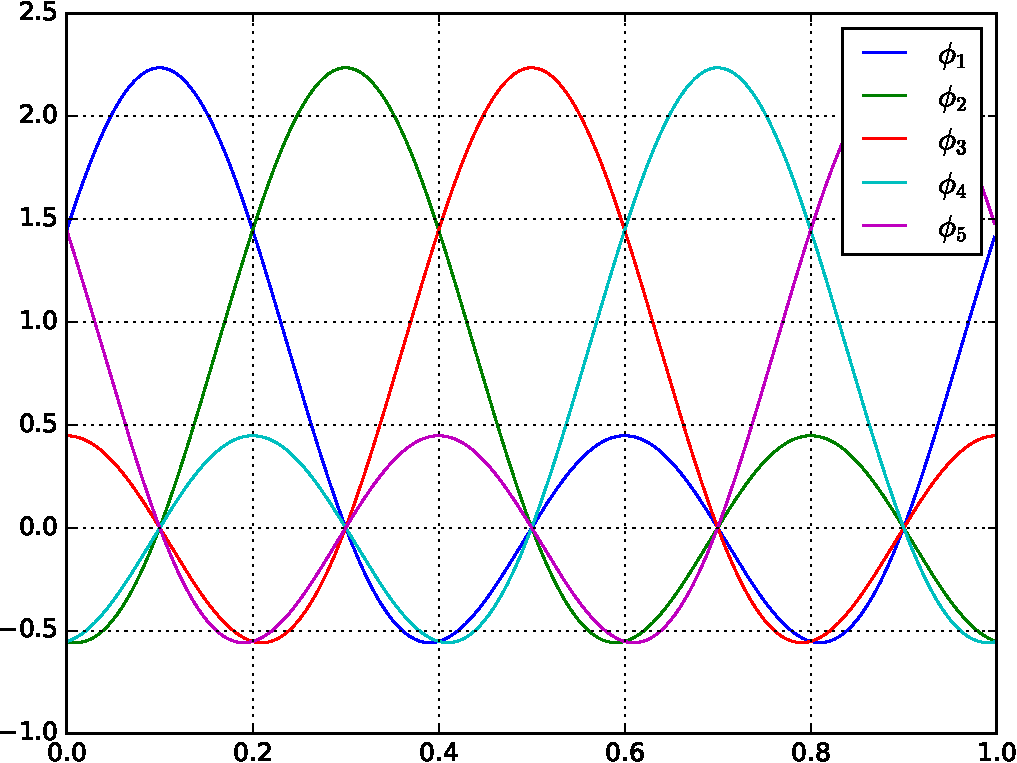
\includegraphics[scale=0.5]{images/plotN_5.pdf}
\end{figure}

Sembarang fungsi periodic $f(x) = f(x+L_{\alpha})$ dapat diekspansi dalam fungsi basis
Lagrange
\begin{equation}
f(x) = \sum_{\alpha}^{N_{\alpha}} c_{\alpha} \phi_{\alpha}(x)
\end{equation}
dengan $c_{\alpha}$ adalah koefisien ekspansi.
Nilai fungsi $f(x)$ pada titik grid $x_{\alpha}$ dapat diperoleh langsung
dari koefisien ekspansi melalui hubungan
$c_{\alpha} = \sqrt{L_{\alpha}/N_{\alpha}}f(x_{\alpha})$.

Ekspansi persamaan Kohn-Sham dengan fungsi basis Lagrange:
\begin{equation}
\psi_{i}(\mathbf{r}) = \sum_{\alpha\beta\gamma}
C^{i}_{\alpha\beta\gamma} \Phi_{\alpha\beta\gamma}(\mathbf{r})
\end{equation}
dengan fungsi basis \cite{Baye2015}
\begin{equation}
\Phi_{\alpha\beta\gamma}(\mathbf{r}) =
\phi_{\alpha}(x)\phi_{\beta}(y)\phi_{\gamma}(z)
\end{equation}

\section{Perhitungan}

Fortran90:
diuji dengan menggunakan kompiler berikut: GFortran, g95, ifort, pgi, dan Sun

Potensial eksternal berupa fungsi Gaussian:
\begin{equation}
V_{\mathrm{ext}}(r) = A\exp(-\alpha r^2)
\end{equation}

\begin{figure}[h]
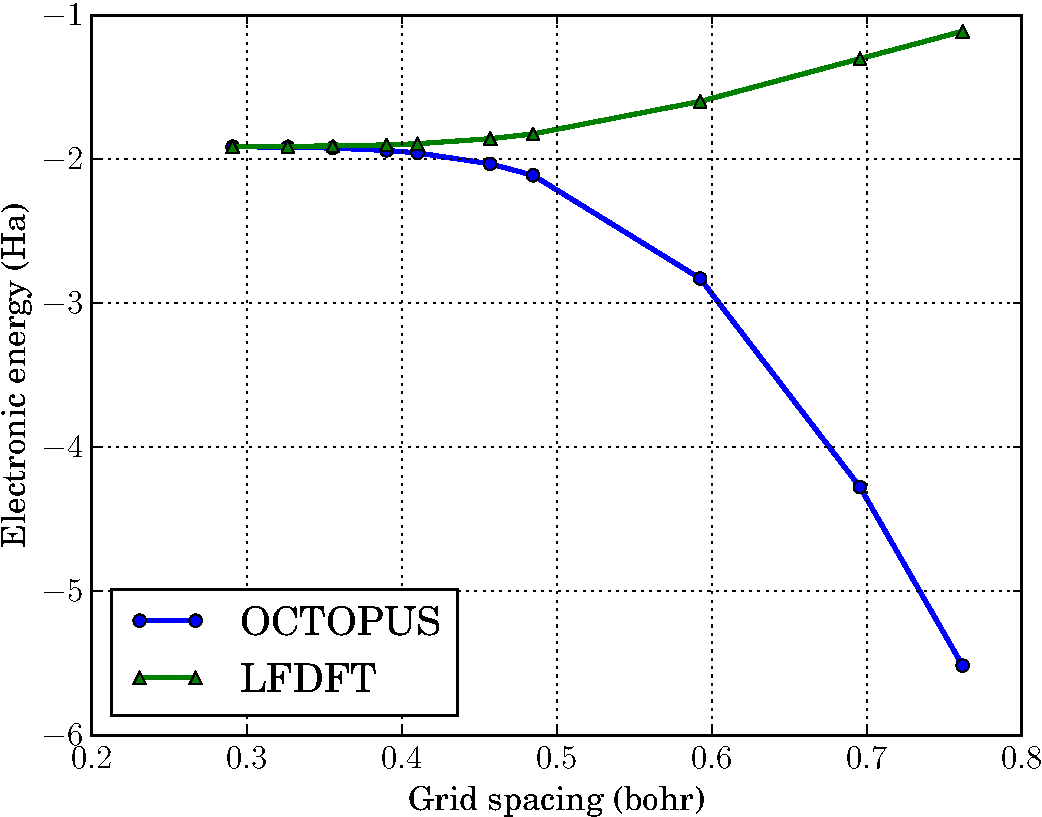
\includegraphics[width=\columnwidth]{images/A_10_alpha_3.pdf}
\end{figure}

Menggunakan bagian lokal dari pseudopotensial HGH
\begin{multline}
V_{\mathrm{ext}}(r) = -\frac{Z_\mathrm{ion}}{r}
\mathrm{erf}\left(\frac{\bar{r}}{\sqrt{2}}\right) +
\exp\left[-\frac{1}{2}\bar{r}^2\right] \\ 
\times
\left[
C_{1} + C_{2}\bar{r}^2 + C_{3}\bar{r}^4 + C_{4}\bar{r}^2
\right]
\end{multline}
dengan $\bar{r} = r/r_{\mathrm{loc}}$

\begin{figure}[h]
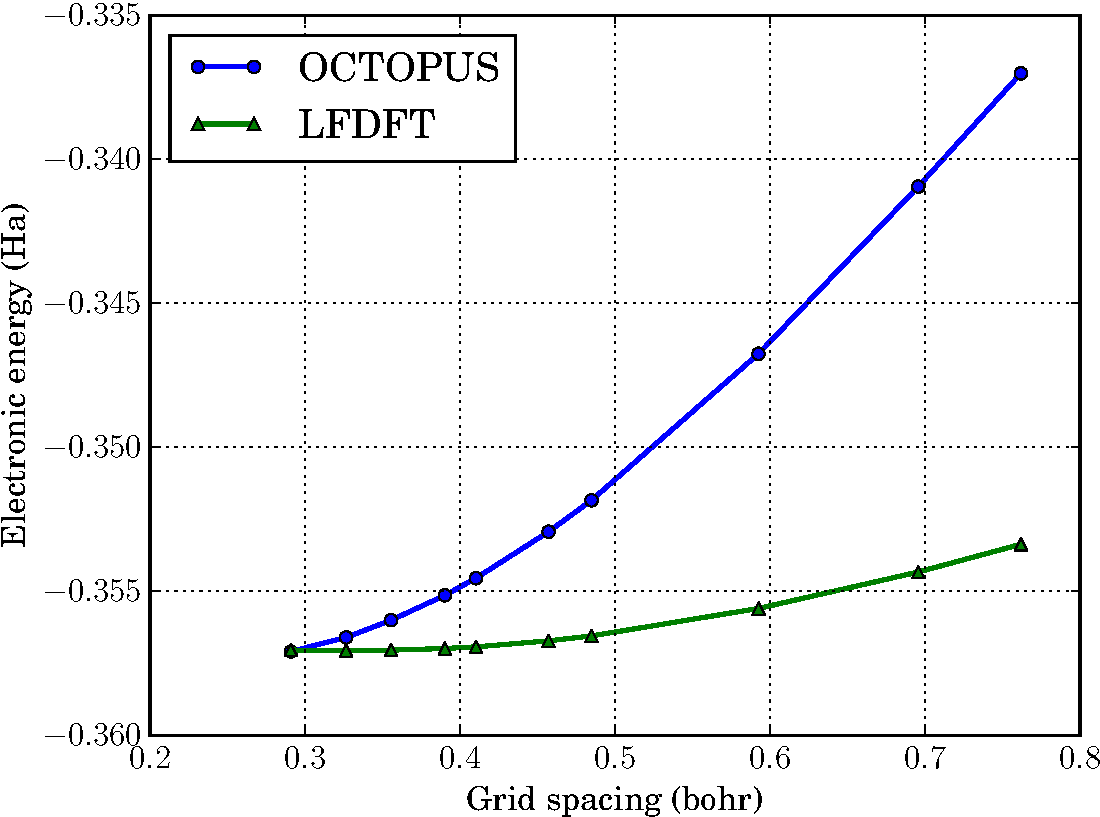
\includegraphics[width=\columnwidth]{images/atom_H.pdf}
\end{figure}

Contoh molekul diatomik: $\ce{H2}$ dan LiH

Visualisasi orbital molekul

\section{Kesimpulan}

Implementasi


\bibliography{LFDFT-v1}

\end{document}


